% Section content template for individual Educative lessons
% This file contains the actual content for a specific section
% Generated from Educative API section content

% Section: Evaluation of a Blob Store's Design
% Section ID: 5348783000387584
% Section Slug: evaluation-of-a-blob-stores-design
% Generated: 2025-12-07T21:38:04.243157

\subsection{Requirements compliance}\label{YF6t9xGZLYhSh4uV6F431}
\\
Let's evaluate how our design helps us achieve our requirements.

\subsubsection{Availability}\label{q4kSKHryY0ZcXXR4hZuwm}
\\
The replication part of our design makes the system available. For reading the data, we keep four replicas for each blob. Having replicas, we can distribute the request load. If one node fails, the other replica node can serve the request. Moreover , our replica placement strategy handles a whole data center failure and can even handle the situation of region unavailability due to natural disasters(Natural disasters include floods, earthquakes, wildfires, tornadoes, nuclear reactor meltdowns, and so on.). We ensure that enough replicas are available at any point in time using our monitoring service, which makes a copy of the data in a timely manner if the number of failed replicas exceeds the specified threshold.
\\
For write requests, we replicate the data within the cluster in a fault-tolerant way and quickly respond to the user, making the system available for write requests.
\\
To keep the manager node available, we keep a backup of its state. In the case of a manager-node failure, we start a new instance of the manager node, initializing it from the saved state.

\subsubsection{Durability}\label{BPqJ9d8xZh6PGTwbAh9p9}
\\
The replication and monitoring services ensure the durability of the data. The data, once uploaded, is synchronously replicated within a storage cluster. If data loss occurs at one node, we can recover the data from the other nodes. The monitoring service monitors the storage disks. If any disk fails, the monitoring service alerts the administrators to change the disk and sends messages to the manager node to copy the content on that disk on to the other available disk or the newly added disk. The manager node then updates the mapping accordingly.

\begin{figure}[htbp]
 \centering
 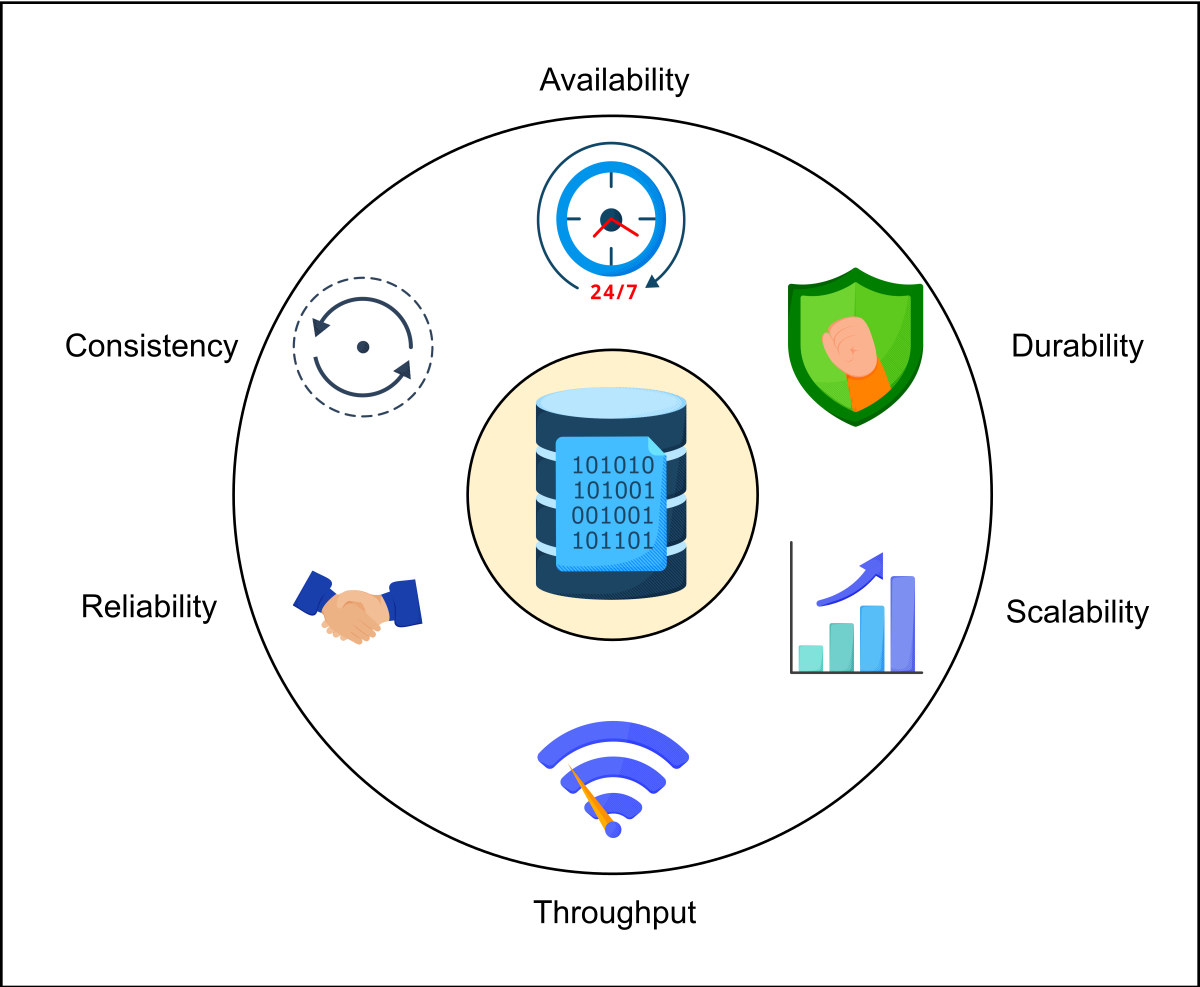
\includegraphics[width=0.5\textwidth]{Images/chapter_20/section_5348783000387584/6274098395480064.png}
 \caption{Guarantees provided by the blob store }
\end{figure}

\subsubsection{Scalability}\label{vpUbMv5RIf6-iDtghfsKN}
\\
The partitioning and splitting of blobs into small-sized chunks helps us scale for billions of blob requests. Blobs are partitioned into separate ranges and served by different partition servers. The partition mappings specify which partition server will serve which particular blob range requests. Partitioning also provides automatic load balancing between partition servers to fulfill the blobs' traffic needs.\\
\strut \\
Our system is horizontally scalable for storage. As need for storage arises, we add more data nodes. At some point, though, our manager node can become a bottleneck. A single manager node can handle 10,000 queries per second (QPS).

\begin{quote}
\textbf{Quiz:}
\textbf{Question 1:} How can we further scale when our manager server hits its limits and we can't improve its computational abilities by vertical scaling?
\textbf{Answer:} We can make two independent instances of our system. Each instance will have its own manager node and a set of data nodes. Deployment of a system similar to ours has been shown to scale up to a few petabytes.

Therefore, making additional instances can help us scale further. For further scaling inside a single instance, we need a new, more  complicated design: "Windows Azure Storage: A Highly Available Cloud
Storage Service with Strong Consistency". .
\end{quote}

\subsubsection{Throughput}\label{0j8qZGd9xrHBjsBkE1S10}
\\
We save chunks of a blob on different data nodes that distribute the requests for a blob to multiple machines. Parallel fetching of chunks from multiple data nodes helps us achieve high throughput.\\
\strut \\
Additionally, caching at different layers--- the client side, front-end servers, and the manager node---improves our throughput and reduces latency.\\

\subsubsection{Reliability}\label{YkP6gdpI_pqaLNETn_YNW}
\\
We achieve reliability through our monitoring techniques. For example, the heartbeat protocol keeps the manager node updated on the status of data nodes. This enables the manager node to request data from reliable nodes only. Furthermore , it takes necessary precautions to ensure reliable service. For example, the failure of a node triggers the manager node to request an additional replica node.
\\
The monitoring services also alert the administrators to change faulty hardware like failed disks or broken network links or switches. To ensure a reliable service, the manager node keeps track of the available space on the disk. If the available space left reaches a certain threshold, an alert is sent to the administrators to add new disks.

\subsubsection{Consistency}\label{1IXXcT47ZNOkW2jGAvP2W}
\\
We synchronously replicate the disk data blocks inside a storage cluster upon a write request, making the data strongly consistent inside the storage cluster. This is done on the user's critical path. We serve the subsequent read requests on this data from the same storage cluster until we have replicated this data in another data center and or on other storage clusters.
\\
After responding to the write request and replicating data within the storage cluster, we asynchronously replicate blobs in the data centers placed far away or in other regions to ensure availability.
\\
We haven't discussed security as a nonfunctional requirement for the blob store. Now , it's your turn to think about how we can implement security to keep the data at rest and in transit safe.
\\
What techniques would you use to make the blob store \textbf{secure}? Write your answer in the widget below.

\textbf{Question:}

What techniques would you use to make the design secure?

\textbf{Reference Answer:}

For data at rest security in a Blob Store, encryption techniques such as AES (Advanced Encryption Standard) can be employed. This involves encrypting the stored data, making it unreadable without the appropriate decryption key.
\\
For data-in-transit security, using HTTPS (Hypertext Transfer Protocol Secure) is crucial as it uses HTTP over SSL/TLS. It encrypts the communication between clients and the Blob Store, preventing unauthorized access and ensuring the confidentiality and add to the integrity of the transmitted data
\\
Role-based access control (RBAC) can be used to regulate user permissions and restrict unauthorized access to sensitive data. Additionally , implementing data integrity checks such as checksums or hash functions will ensure that data remains unchanged and uncorrupted during storage and transmission.

\subsection{Conclusion}\label{NSrQhHWFjBArmIPQxI7ew}
\\
We saw that a blob store is designed to store large-sized and unstructured data. A blob store helps applications store images, videos, audio, and so on. Nowadays , it's used by many applications like YouTube, Facebook, Instagram, Twitter, and more. We designed a system where users can perform a blob store's basic function. Lastly
, we evaluated our design based on our non-functional requirements.

% End of section content